\documentclass[11pt]{article}
\usepackage[margin=0.9in]{geometry}
\usepackage{amsmath,amssymb}
\usepackage{tikz}
\usepackage{pgfplots}
\pgfplotsset{compat=1.16}
\usetikzlibrary{positioning,arrows.meta,fit,backgrounds,calc}
\usepackage{booktabs}
\usepackage{xcolor}
\usepackage{enumitem}
\usepackage{mdframed}

\definecolor{ink}{HTML}{1f2933}
\definecolor{accent}{HTML}{2563a8}
\definecolor{warm}{HTML}{c0552b}
\definecolor{good}{HTML}{2e7d5b}
\definecolor{soft}{HTML}{e8eef5}

\newcommand{\norm}[1]{\left\lVert #1 \right\rVert}
\newcommand{\R}{\mathbb{R}}

\newmdenv[linecolor=accent,linewidth=1pt,backgroundcolor=soft,
  roundcorner=4pt,innertopmargin=8pt,innerbottommargin=8pt,
  innerleftmargin=10pt,innerrightmargin=10pt]{keybox}

\title{\textbf{Compress the Response, Not the Data}\\[2pt]
\large Three everyday pictures of response-preserving aggregation}
\author{}
\date{}

\begin{document}
\maketitle
\vspace{-3.2em}

\begin{center}\rule{0.5\textwidth}{0.4pt}\end{center}

\section*{The one idea}

Every compression has the same shape: take data $x$, fold it down to a small
code $z$, unfold it back to an approximation $\tilde x$.
\[
x \;\xrightarrow{\ \text{fold }E\ }\; z \;\xrightarrow{\ \text{unfold }U\ }\; \tilde x .
\]
The usual goal is $x \approx \tilde x$. But often we do not care about $x$
itself --- we care about what a \emph{system} does to it. If a matrix $A$ turns
input into the thing we actually observe, the real goal is
\[
\boxed{\,A x \approx A\tilde x\,}
\qquad\Longleftrightarrow\qquad
A\,(I - UE)\,x \approx 0 .
\]
Two inputs may be far apart yet produce the same output; two may be close yet
produce different outputs. \textbf{Merge by response, not by appearance.} That
single sentence is the whole method. The traffic version is identical: do not
insist the OD table $d$ be reconstructed; insist that the link flow
$v = Hd$ be preserved, where $H = B^{\!\top}R$ is the OD-to-link response.

\begin{center}
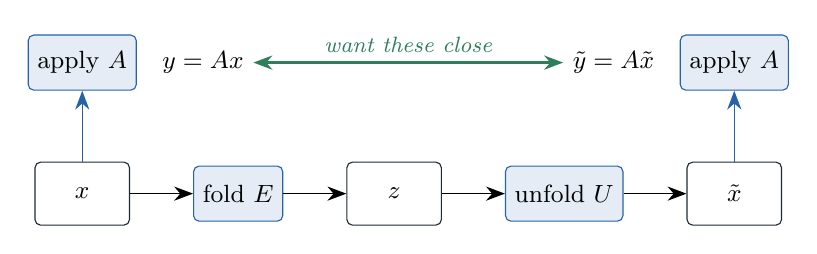
\begin{tikzpicture}[
  font=\small,
  box/.style={draw=ink,rounded corners=2pt,minimum height=8mm,minimum width=12mm,fill=white},
  op/.style={draw=accent,fill=accent!12,rounded corners=2pt,minimum height=7mm},
  >={Stealth[length=2.4mm]}]
  \node[box] (x) {$x$};
  \node[op,right=8mm of x] (E) {fold $E$};
  \node[box,right=8mm of E] (z) {$z$};
  \node[op,right=8mm of z] (U) {unfold $U$};
  \node[box,right=8mm of U] (xt) {$\tilde x$};
  \draw[->] (x)--(E); \draw[->] (E)--(z); \draw[->] (z)--(U); \draw[->] (U)--(xt);
  % response branch
  \node[op,above=9mm of x] (A1) {apply $A$};
  \node[op,above=9mm of xt] (A2) {apply $A$};
  \node[right=2mm of A1] (y1) {$y=Ax$};
  \node[left=2mm of A2] (y2) {$\tilde y=A\tilde x$};
  \draw[->,accent] (x)--(A1);
  \draw[->,accent] (xt)--(A2);
  \draw[<->,good,thick] (y1.east) -- node[above,font=\footnotesize\itshape,text=good]{want these close} (y2.west);
\end{tikzpicture}
\end{center}

\section*{Example 1 --- Image compression: merge by response}

A tiny grayscale image, four pixels. Group them into two super-pixels by
averaging (the fold $E$), then paint each group back with its average (the
unfold $U$):
\[
E=\tfrac12\begin{bmatrix}1&1&0&0\\0&0&1&1\end{bmatrix},
\qquad
U=\begin{bmatrix}1&0\\1&0\\0&1\\0&1\end{bmatrix}.
\]

\noindent
\begin{minipage}[t]{0.48\textwidth}
\centering
\textbf{Good grouping.}\\[2pt]
$x=(10,12,80,82)$ --- adjacent pixels already alike.
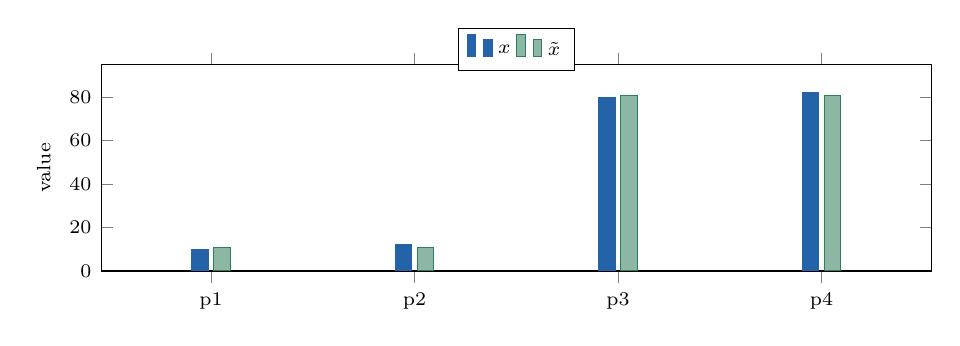
\begin{tikzpicture}
\begin{axis}[ybar,width=\linewidth,height=4.2cm,symbolic x coords={p1,p2,p3,p4},
  xtick=data,ymin=0,ymax=95,bar width=6pt,enlarge x limits=0.18,
  legend style={font=\scriptsize,at={(0.5,1.18)},anchor=north,legend columns=2},
  tick label style={font=\scriptsize},ylabel style={font=\scriptsize},
  ylabel={value}]
\addplot[fill=accent,draw=accent] coordinates {(p1,10)(p2,12)(p3,80)(p4,82)};
\addplot[fill=good!55,draw=good] coordinates {(p1,11)(p2,11)(p3,81)(p4,81)};
\legend{$x$,$\tilde x$}
\end{axis}
\end{tikzpicture}\\[-1pt]
{\footnotesize error $x-\tilde x=(-1,1,-1,1)$ --- tiny.}
\end{minipage}\hfill
\begin{minipage}[t]{0.48\textwidth}
\centering
\textbf{Bad grouping.}\\[2pt]
$x=(10,80,12,82)$ --- same fold, but it mixes dark with bright.
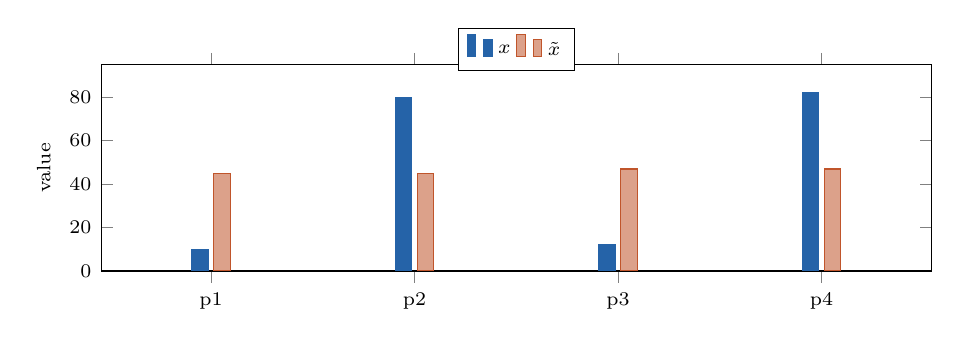
\begin{tikzpicture}
\begin{axis}[ybar,width=\linewidth,height=4.2cm,symbolic x coords={p1,p2,p3,p4},
  xtick=data,ymin=0,ymax=95,bar width=6pt,enlarge x limits=0.18,
  legend style={font=\scriptsize,at={(0.5,1.18)},anchor=north,legend columns=2},
  tick label style={font=\scriptsize},ylabel style={font=\scriptsize},
  ylabel={value}]
\addplot[fill=accent,draw=accent] coordinates {(p1,10)(p2,80)(p3,12)(p4,82)};
\addplot[fill=warm!55,draw=warm] coordinates {(p1,45)(p2,45)(p3,47)(p4,47)};
\legend{$x$,$\tilde x$}
\end{axis}
\end{tikzpicture}\\[-1pt]
{\footnotesize error $=(-35,35,-35,35)$ --- ruinous.}
\end{minipage}

\vspace{4pt}
The fold matrix is the same in both panels. The only difference is
\emph{which} pixels got merged. \textbf{Lesson: aggregate things that respond
alike, not things that sit next to each other.}

\section*{Example 2 --- Equalizer: preserve what is heard}

Four frequency-band volumes feed a speaker:
$x=(\text{bass}_1,\text{bass}_2,\text{mid},\text{treble})$. Nobody hears $x$.
What reaches the ear is the speaker response $y = A x$, where column
$A_{:,k}$ is how band $k$ moves the output. If two bands push the output the
same way, $A_{:,1}\approx A_{:,2}$, they can be merged into one super-band
with no audible loss --- even though they are different inputs.

\begin{center}
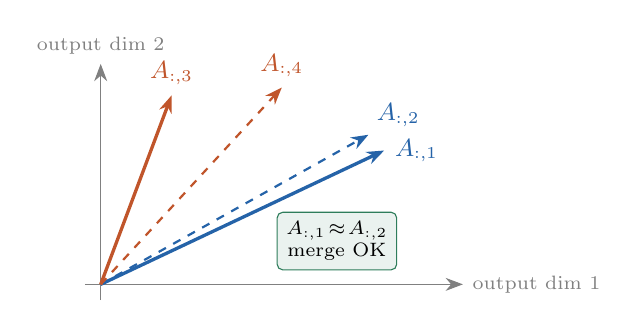
\begin{tikzpicture}[font=\small,>={Stealth[length=2.2mm]},scale=1.0]
  \draw[->,gray] (-0.2,0)--(4.6,0) node[right,font=\scriptsize]{output dim 1};
  \draw[->,gray] (0,-0.2)--(0,2.8) node[above,font=\scriptsize]{output dim 2};
  % cols 1,2 nearly parallel
  \draw[->,accent,very thick] (0,0)--(3.6,1.7) node[right]{$A_{:,1}$};
  \draw[->,accent,thick,dashed] (0,0)--(3.4,1.9) node[above right=-1pt]{$A_{:,2}$};
  % cols 3,4 different
  \draw[->,warm,very thick] (0,0)--(0.9,2.4) node[above]{$A_{:,3}$};
  \draw[->,warm,thick,dashed] (0,0)--(2.3,2.5) node[above]{$A_{:,4}$};
  \node[draw=good,rounded corners=2pt,fill=good!10,font=\scriptsize,
        align=center] at (3.0,0.55) {$A_{:,1}\!\approx\!A_{:,2}$\\merge OK};
\end{tikzpicture}
\end{center}

\noindent The target is not $x\approx\tilde x$ but $Ax\approx A\tilde x$, i.e.
$A(I-UE)x\approx 0$. This is exactly the traffic statement, term for term:

\begin{center}
\small
\begin{tabular}{ll}
\toprule
Equalizer & Traffic \\
\midrule
$x$: band inputs & $d$: OD demand \\
$A$: speaker response & $H=B^{\!\top}R$: OD-to-link response \\
$y=Ax$: sound heard & $v=Hd$: link flow \\
merge similar bands & merge response-similar zones \\
keep the sound undistorted & keep corridor flow undistorted \\
\bottomrule
\end{tabular}
\end{center}

\section*{Example 3 --- Student grades: the low-rank code behind SVD}

A student$\times$course score matrix. The first two courses behave like
math/physics, the last two like literature/history:
\[
X=\begin{bmatrix}
90&92&30&28\\ 88&91&32&31\\ 25&27&85&88\\ 28&30&82&86
\end{bmatrix}.
\]
Four columns, but really only two abilities drive everything: a STEM score and
a humanities score. The effective rank is $2$, not $4$.

\begin{center}
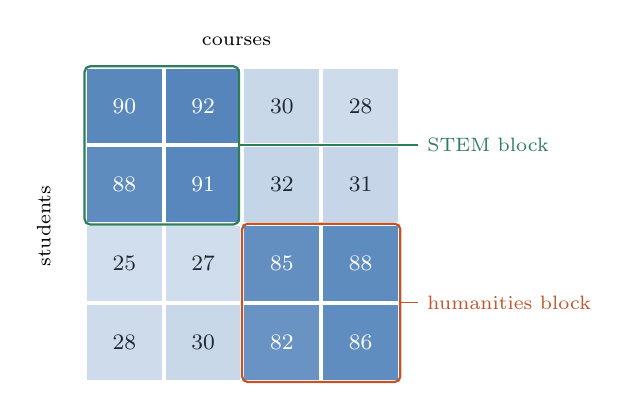
\begin{tikzpicture}[font=\footnotesize]
  \foreach \r [count=\ri from 0] in {{90,92,30,28},{88,91,32,31},{25,27,85,88},{28,30,82,86}} {
    \foreach \v [count=\ci from 0] in \r {
      \pgfmathtruncatemacro{\shade}{\v*0.85}
      \pgfmathparse{\v>55 ? "white" : "ink"}\edef\txtcol{\pgfmathresult}
      \fill[accent!\shade!white] (\ci,-\ri) rectangle ++(0.95,0.95);
      \node[text=\txtcol] at (\ci+0.475,-\ri+0.475) {\v};
    }
  }
  \node[rotate=90,font=\scriptsize] at (-0.55,-1.05) {students};
  \node[font=\scriptsize] at (1.9,1.3) {courses};
  \draw[good,thick,rounded corners=2pt] (-0.03,0.98) rectangle (1.93,-1.03);
  \draw[warm,thick,rounded corners=2pt] (1.97,-1.02) rectangle (3.98,-3.03);
  \draw[good] (1.93,-0.02) -- (4.2,-0.02);
  \node[good,font=\scriptsize,right] at (4.2,-0.02) {STEM block};
  \draw[warm] (3.98,-2.02) -- (4.2,-2.02);
  \node[warm,font=\scriptsize,right] at (4.2,-2.02) {humanities block};
\end{tikzpicture}
\end{center}

\noindent The SVD reads off those two abilities automatically:
\[
X \approx \underbrace{U_2\Sigma_2}_{\text{decoder}}\ \underbrace{V_2^{\!\top}}_{\text{encoder}} .
\]
$V_2^{\!\top}$ encodes four course scores into two latent ability scores;
$U_2\Sigma_2$ decodes them back into the grade pattern. SVD is the
\emph{optimal} low-rank fold/unfold --- but its two ``abilities'' are abstract
mixtures, not nameable courses.

\section*{Bridge: from these pictures to super-zones}

Super-zone aggregation is the \emph{interpretable} cousin of SVD. The fold is
the OD aggregation $E=Q^{\!\top}=(S\otimes S)^{\!\top}$ and the unfold is
$U$, so the compressed demand is $\tilde d = U Q^{\!\top} d$.\footnote{The
unfolding operator $U$ and the SVD left factor $U_s$ are different objects;
they share a letter only by convention.} Both are fold/unfold pipelines:
\[
\text{SVD:}\quad H \approx U_s\Sigma_s V_s^{\!\top}
\qquad\text{vs.}\qquad
\text{super-zone:}\quad d \to Q^{\!\top}d \to U Q^{\!\top} d .
\]
We choose the zone map $S$ so the interpretable fold tracks the optimal one on
the corridors that matter:
\[
\boxed{\,H\,U\,Q^{\!\top} \;\approx\; U_s\Sigma_s V_s^{\!\top}
\quad\Longleftrightarrow\quad
H d \;\approx\; H\,U\,Q^{\!\top} d \text{ on the dominant corridor modes.}\,}
\]
SVD says how many modes exist (the rank floor); the super-zones give names to
them (geographic groups) while preserving the same dominant response.

\begin{keybox}
\textbf{The talking script.} Image compression shows that fold/unfold is just
merging similar items and expanding them back. The equalizer shows the thing
to preserve is not the input but the system response $Ax$. SVD gives the
optimal low-rank fold/unfold and tells you how many modes are real. Traffic
demand compression is the same logic with names attached: $Q^{\!\top}$ folds
the OD table, $U$ unfolds it, $H=B^{\!\top}R$ is the system response. We never
demand that the OD table be preserved --- only that $Hd$ and $H U Q^{\!\top}d$
agree on the leading low-rank corridor modes.
\end{keybox}

\end{document}
